
\begin{frame}{NP effect (LMM)}
\only<1>{
	\begin{flushright}
		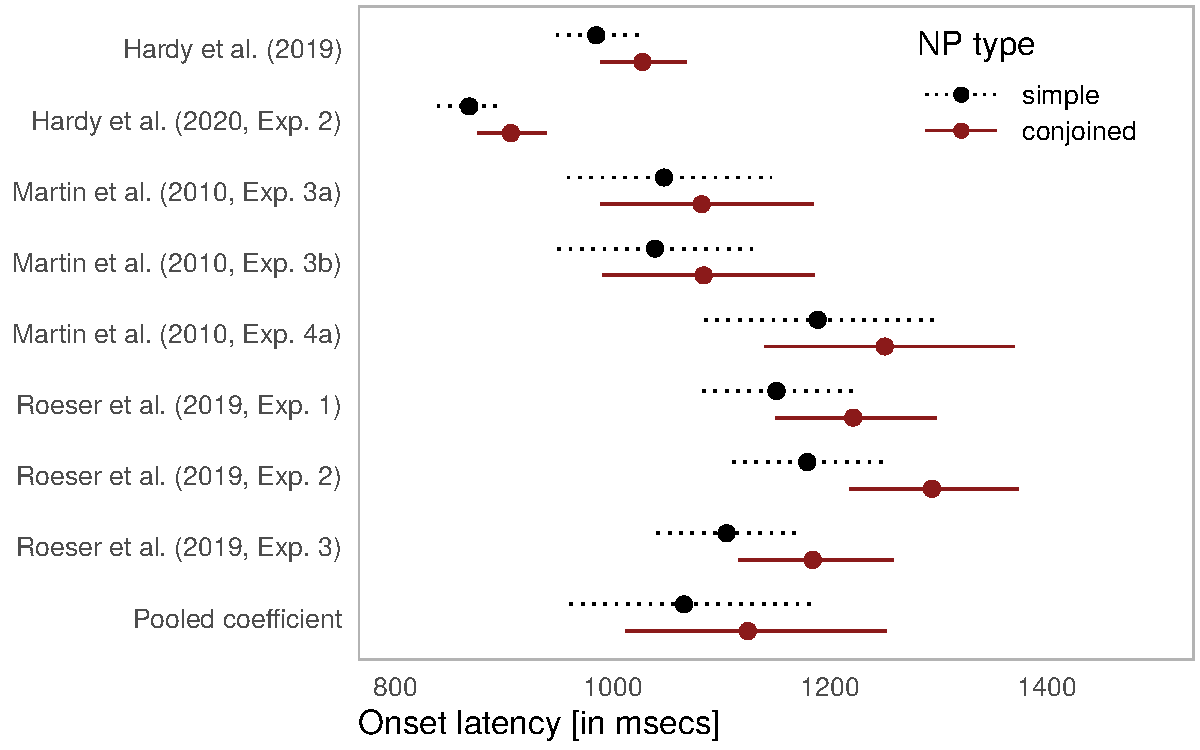
\includegraphics[scale=.5]{NPmeta.pdf}
	\end{flushright}
}
\only<2>{
	\begin{flushright}	
		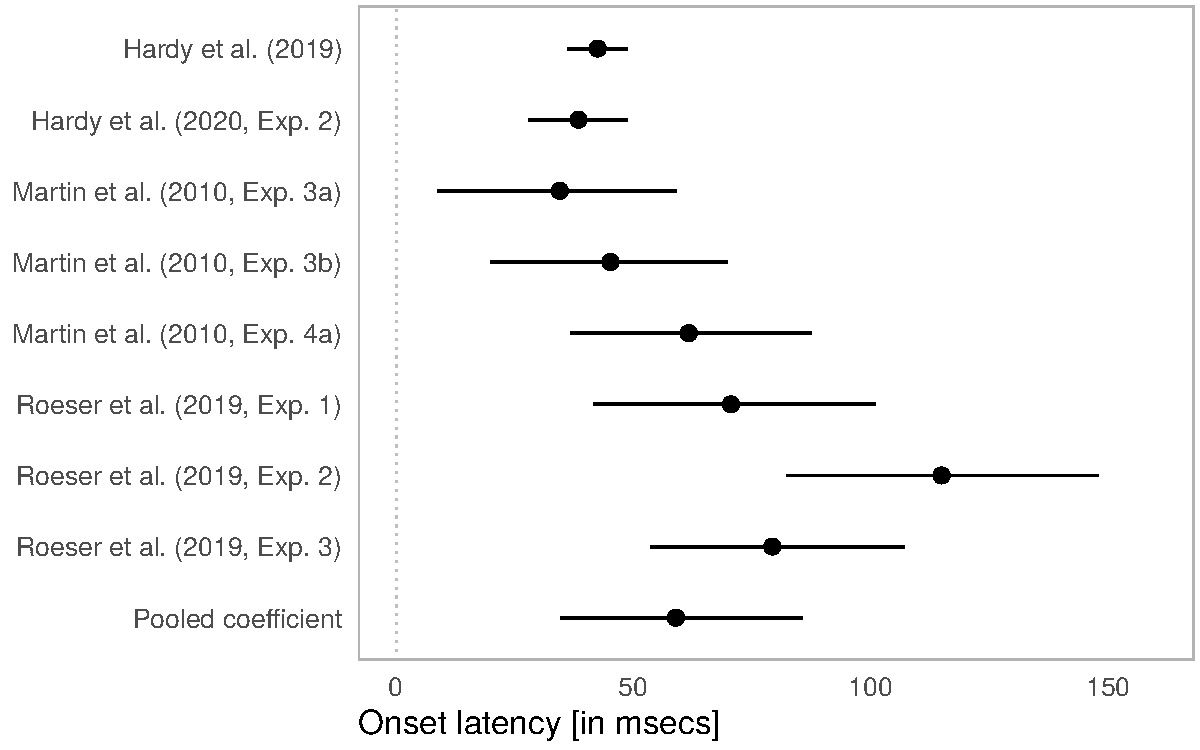
\includegraphics[scale=.5]{NPmetadiff.pdf}
	\end{flushright}
}
\end{frame}



\begin{frame}{Model comparisons}

\only<1>{
	\begin{scriptsize}
		% latex table generated in R 4.0.2 by xtable 1.8-4 package
		% Tue Aug 18 15:17:51 2020
		\begin{table}[ht]
			\centering
			\caption{\scriptsize{Predictive performance estimated as the \textit{expected log predictive density} ($\widehat{elpd}$) \parencite{vehtari2015pareto, vehtari2017practical}. Models are ordered by predictive performance (model with highest predictive performance in top row)}. Standard error in parentheses.}
			\begin{tabular}{lrrl}
				\toprule
				Models & $\updel\widehat{elpd}$ & $\widehat{elpd}$ & Description \\ [1ex]
				\midrule
				MoG-1 &  & & Mixing proportions by NP-type \\ [1ex]
				MoG-0 &  & & Null model (no NP difference) \\ [1ex]
				LMM-1 &  & & Slowdown for conjoined NPs \\ [1ex]
				LMM-0 &  & & Null model (no NP difference) \\ [1ex]
				LMM-2 & {\color{white}-3,537 (214)} & {\color{white}-205,022 (307)} & Larger variance for conjoined NPs \\ [1ex]
				\bottomrule
			\end{tabular}\\
			\textit{Note.} LMM = Linear mixed effects model; MoG = Mixture of Gaussians 
		\end{table}
	\end{scriptsize}
}

\only<2>{
	\begin{scriptsize}
		% latex table generated in R 4.0.2 by xtable 1.8-4 package
		% Tue Aug 18 15:17:51 2020
		\begin{table}[ht]
			\centering
			\caption{\scriptsize{Predictive performance estimated as the \textit{expected log predictive density} ($\widehat{elpd}$) \parencite{vehtari2015pareto, vehtari2017practical}. Models are ordered by predictive performance (model with highest predictive performance in top row)}. Standard error in parentheses.}
			\begin{tabular}{lrrl}
				\toprule
				Models & $\updel\widehat{elpd}$ & $\widehat{elpd}$ & Description \\ [1ex]
				\midrule
				MoG-1 & -- & -201,486 (176) & Mixing proportions by NP-type \\ [1ex]
				MoG-0 & -15 (8) & -201,500 (176)  & Null model (no NP difference) \\ [1ex]
				LMM-1 & -1,006 (97) & -202,492 (214) & Slowdown for conjoined NPs \\ [1ex]
				LMM-0 & -1,192 (92) & -202,678 (212) & Null model (no NP difference) \\ [1ex]
				LMM-2 & -3,537 (214) & -205,022 (307) & Larger variance for conjoined NPs \\ [1ex]
				\bottomrule
			\end{tabular}\\
			\textit{Note.} LMM = Linear mixed effects model; MoG = Mixture of Gaussians 
		\end{table}
	\end{scriptsize}
}

\only<3>{
\begin{scriptsize}
% latex table generated in R 4.0.2 by xtable 1.8-4 package
% Tue Aug 18 15:17:51 2020
	\begin{table}[ht]
	\centering
	\caption{\scriptsize{Predictive performance estimated as the \textit{expected log predictive density} ($\widehat{elpd}$) \parencite{vehtari2015pareto, vehtari2017practical}. Models are ordered by predictive performance (model with highest predictive performance in top row)}. Standard error in parentheses.}
		\begin{tabular}{lrrl}
		\toprule
		Models & $\updel\widehat{elpd}$ & $\widehat{elpd}$ & Description \\ [1ex]
		\midrule
		\rowcolor{yellow!40!white}MoG-1 & -- & -201,486 (176) & Mixing proportions by NP-type \\ [1ex]
  		MoG-0 & -15 (8) & -201,500 (176)  & Null model (no NP difference) \\ [1ex]
 		\rowcolor{yellow!40!white}LMM-1 & -1,006 (97) & -202,492 (214) & Slowdown for conjoined NPs \\ [1ex]
  		LMM-0 & -1,192 (92) & -202,678 (212) & Null model (no NP difference) \\ [1ex]
 		LMM-2 & -3,537 (214) & -205,022 (307) & Larger variance for conjoined NPs \\ [1ex]
		\bottomrule
		\end{tabular}\\
		\textit{Note.} LMM = Linear mixed effects model; MoG = Mixture of Gaussians 
	\end{table}
\end{scriptsize}
}
\end{frame}



\begin{frame}{Probability of long latencies (MoG)}

	\begin{flushright}
		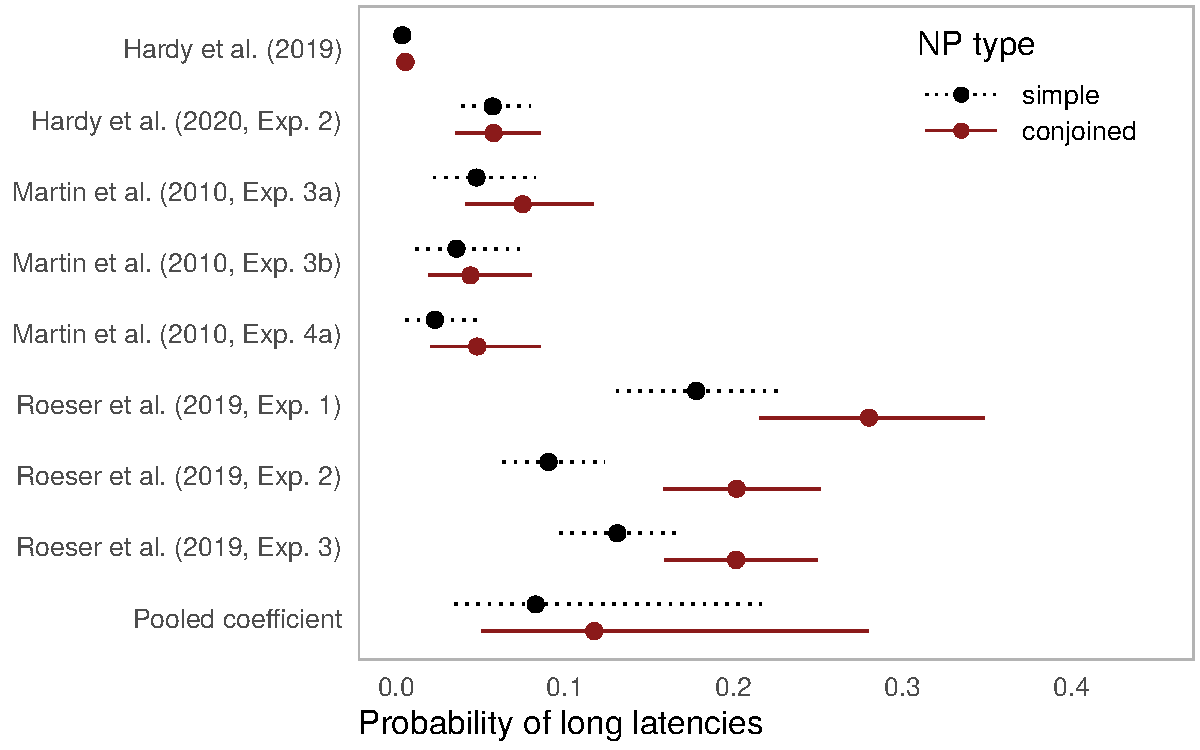
\includegraphics[scale=.5]{mogmeta.pdf}
	\end{flushright}


\end{frame}